\section{Mobile Parsing R-CNN}
\label{section3}

In this section, we address the design choice of different parts inside our model, which we call Mobile Parsing R-CNN. In general, the model's design follows the Parsing R-CNN model, the winner solution of the COCO 2018 Challenge DensePose Estimation task, but with different modifications in different parts.

\subsection{Backbone}

While there are many different possible designs of a backbone network, we target efficient models with a block structure as that in MobileNetV1 and V2 \cite{mobilenetv1, mobilenetv2} (depth-wise separable convolutions and inverted residuals with linear bottlenecks). This base block is the foundation for most efficient backbones used today, which were selected for evaluation as the backbone of the improved model. 
Let us list various architectures we use in our experiments:
\begin{itemize}
    \item \textbf{MobileNetV3}.  \cite{mobilenetv3} applies neural architecture search (NAS) and improves MobileNetV2 by adopting Squeeze and excitation block for channel-wise attention and non-linearities like h-sigmoid and h-swish;
    \item \textbf{MixNet}. \cite{mixnet} develops a multi-kernel variant of MobileNetV2, i.e., depth-wise convolutions consisting of convolutions with different kernel sizes;
    \item \textbf{Differentiable NAS} considers the problem of finding neural architecture in a differentiable way by carefully designing search space. We consider the following models, obtained using the differentiable NAS procedure: MnasNet \cite{mnasnet}, FBNet \cite{fbnet}, Single-Path\cite{spnasnet};
    \item \textbf{EfficientNets} from \cite{efficientnetb} appear to be one of the first architectures, obtained using AutoML approaches for image classification, and achieve a good compromise between the accuracy on a classification task and the number of the parameters of the network. \cite{efficientnetb} shows that one can apply a power-law scaling of width as a function of depth. Later EfficientNets were customized for Google's Edge TPUs \cite{efficientnete} using MNAS framework \cite{mnasnet};
    \item \textbf{CondConv}. Traditional convolutional layers have the kernel weights fixed once they are trained. CondConv \cite{condconv} applies a linear combination of several kernels (a mixture of experts) with weights generated dynamically by another network based on the input. While the original work is devoted to the classification task, we explore this \textit{``dynamic''} approach combined with EfficientNets on the DensePose task.
\end{itemize}

\subsection{Neck}

The main challenge in the object detection pipeline is to be able to detect objects of different scales. Earlier detectors predict objects based on features extracted from different levels of the backbone. Later, feature pyramid network (FPN \cite{fpn}) proposes to integrate features in a top-down manner to enrich fine-grained features from the lowest level of feature pyramid with semantically rich information from deeper layers. While the original work \cite{fpn} considers only the top-down pathway for information aggregation, later works also add cross-scale connections between the feature levels. In this work, we make use of bidirectional FPN (BiFPN \cite{bifpn}) for multi-scale feature fusion, which outperforms its recent counterparts in object detection tasks (see \cite{bifpn}), while remaining light-weight and fast. It is partly achieved by using separable convolutions inside.

\subsection{Densepose head}

We increase the region of interest (RoI) resolution for the DensePose head from $14\times14$ to $32\times32$, as it was suggested in \cite{parsing}.

While the original network uses 8 convolutions layers in the DensePose head, we, instead, similar to \cite{parsing}, use the atrous spatial pyramid pooling (ASPP) \cite{aspp} module, followed by 4 convolutional layers. Also, we omit the non-local convolutional layer \cite{nonlocal} between ASPP and convolutional layers in order not to increase the latency of the network because it performs pixel to pixel comparisons resulting in $O(n^2)$ operations, where $n$ is the number of pixels.

Finally, the DensePose predictions happen on the finest level from the feature pyramid as in \cite{parsing}, while box/class predictions happen on all levels.

\subsection{Quantization of backbone layers}
\label{quant}

We proposed the quantization procedure for Parsing R-CNN based on quantization aware training tools provided by PyTorch. 
First of all, it is necessary to patch the existing network architecture. Considering the whole network operates with quantized tensors, we should find intermediate parts where floating-point tensors are crucial to obtain satisfactory results.
\begin{enumerate}
    \item RPN classification and regression heads use a $3\times3$ convolutional layer to produce a shared hidden state from which one $1\times1$ convolutional layer predicts objectness logits for each anchor, and another one predicts bounding-box deltas specifying how to refine the anchor coordinates to get a final object proposal. These layers work with quantized feature tensors, but for correct calculation of RPN proposals, predicted objectness logits and anchor deltas are dequantized after inference of bounding box predictor.
    \item To perform accurate RoI pooling, it is necessary first to dequantize input features, apply pooling, and then quantize features back.
    % \item To perform accurate box pooling, it is necessary to dequantize input features. In that case, RoI pooling would work with floating-point features and RPN proposals. After this operation, we quantize cropped feature tensors before passing them to the following layers.
\end{enumerate}

The second step is fusion. We fuse each convolutional and linear layer, followed by batch normalization and activation to one atomic layer. That is needed to save on memory access while also improving the operations' numerical accuracy.
The third step is to run the quantization aware training of the patched and fused model.
% The last step is to perform an evaluation of the resulted model.

During the second and third steps, we run into design obstacles that are described below.

In BiFPN architecture, we collect features before point-wise linear convolutions using pre-forward hooks. This allows us to link to this layer's input rather than to the output of the input provider. But quantization tools implemented in the PyTorch framework at this stage do not allow this to be done. We proposed a mechanism that preserves pre- and post- forward hooks during fusion and preparation for quantization and does not harm the quality of the quantization process itself. The diagram of the proposed mechanism is in Fig.~\ref{fig:preserve_hooks}.

\begin{figure}[!hbtp]
\centering
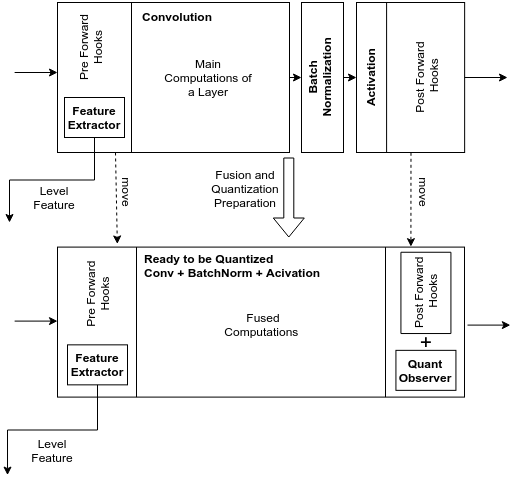
\includegraphics[width=0.4\textwidth]{Figures/densepose/diagram.png}
\caption{The feature collection scheme for quantized models.}
\label{fig:preserve_hooks}
\end{figure}